% !TEX root = ../toptesi-scudo-example.tex
% !TEX encoding = UTF-8 Unicode
%***********************************************************************
%*********************************** First Chapter 

%***********************************************************************
%\cite{lamport1994latex, hertel2010writing}.
%Please see appendix~\ref{Appendix1}.
%***********************************************************************



\chapter{Introduzione}
\label{cap:intro}
\graphicspath{{Pictures/}}


%-----------------------------------------------------------------------
\section{Ambito del lavoro}
\label{sez:ambito}

L'ambito di riferimento di questo lavoro è l'analisi e la trasformazione di segnali digitali, con particolare riferimento alle tecniche di filtraggio in frequenza e alla loro implementazione in ottica di risposta immediata del sistema al segnale ({\it real time signal processing}).

Il presente lavoro è legato al disegno dell'infrastruttura elettronica preposta alla rilevazione dei segnali elettrici derivanti da un esperimento di elettrofisiologia con l'obiettivo di registrare l'attività di uno popolazione di neuroni coltivati {\it in vitro} sopra un array ad alta densità di transistor CMOS. La rilevazione del segnale elettrico dai neuroni con tecnologia {\it a contatto}, con il vantaggio di non interferisce invasivamente con il materiale biologico, impone d'altra parte diverse nuove problematiche di {\it qualità del segnale}, ad esempio la risoluzione spaziale e il rumore di fondo.

A partire dal seminale lavoro di \cite{Hodgkin1952} infatti, la natura e i meccanismi alla base della generazione di segnali elettrici da parte di cellule neuronali sono noti, così come sono disponibili modelli quantitavi che riproducono con buona approssimazione la forma degli impulsi osservati. D'altra parte, l'osservazione di una popolazione reale di cellule nel loro ambiente fisiologico con tecnologie che misurano quantità medie richiede la formulazione di ipotesi sugli effetti di rumore ambientali, dell'interazione reciproca tra le cellule oltre che del rumore insito nella tecnologia di rilevazione.

Tali ipotesi si concretizzano nell'esperimento in questione, nel disegno di un filtro in frequenza del segnale osservato e le successive elaborazioni del segnale filtrato. In particolare, nel filtro risulta definita la banda di frequenza nella quale si attende il segnale ({\it passband}) e quali siano invece le frequenze da abbattere in intensità perché legate a frequenze di rumore ({\it stopband}). Le successive elaborazioni del segnale filtrato nell'esperimento Neurochip riguardano invece la gestione della forte correlazione spaziale tra sensori vicini che permette una miglior identificazione dei picchi di potenziale significativi {\it spike sorting}.



%-----------------------------------------------------------------------
\section{Obiettivi del lavoro}
\label{sez:obiettivo}

A partire dai parametri di un filtro in frequenza disegnato per l'esperimento Neurochip, il presente lavoro:
\begin{itemize}
 \item indaga gli effetti spettrali del campionamento e del rumore sul filtro;
 \item propone e confronta due algoritmi di implementazione del filtro;
 \item simula l'effetto del filtro su un segnale di prova con e senza rumore;
 \item simula l'effetto nel dominio delle frequenze delle successive elaborazioni del segnale filtrato (algoritmo PCA).
\end{itemize}
Le simulazioni e gli algoritmi implementativi analizzati sono stati sviluppati e simulati con un linguaggio di programmazione ad alto livello\footnote{Matlab.}.


%-----------------------------------------------------------------------
\section{Segnali elettrici del sistema nervoso}

Gli organismi di molti esseri viventi sono dotati di un sistema di trasmissione delle informazioni largamente basato su segnali di natura elettrica, chiamato sistema nervoso. La terminologia utilizzata nel campo delle neuroscienze fa spesso riferimento all'idea di tessuto, rete, circuito per la presenza di diversi elementi biologici interconnessi. Il profilo elettrico dei segnali scambiati caratterizza un ampio spettro di attività che vanno dagli stimoli motori più semplici, fino a più evolute funzioni celebrali.

Data la relativa facilità di rilevazione dell'attività elettrica lungo le fibre nervose, rispetto alla complessità sia di rilevazione, che di comprensione delle attività che si svolgono nel sistema nervoso centrale ed in particolare a livello encefalico, la propagazione del segnale elettrico attraverso il sistema nervoso periferico è stata il primo interesse dell'elettrofisiologia. In tale ambito sono stati applicati modelli di propagazione e diffusione di un segnale elettrico attraverso una rete di cavi. Il materiale biologico legato a tale funzione è stato perciò analizzato con riguardo anche alle sue proprietà elettriche; la resistività dei tessuti e gli schemi elettrici assimilabili per spiegare la forma degli impulsi elettrici osservati. Una breve rassegna di tali proprietà viene riporata nella successiva sezione \ref{sez:Fisiologia} con riferimento ad un singolo neurone.

L'aspetto più complesso legato all'elaborazione o modulazione del segnale oltre che alla sua trasmissione è stato per la prima volta descritto con precisione dal seminale contributo di \cite{Hodgkin1952}. Con un impianto di sonda nell'assone di una specie di calamaro gigante, l'esperimento ha gettato luce sui meccanismi di generazione del segnale elettrico, in base ai quali gli autori hanno formulato un modello matematico che replica con buon adattamento la forma dell'impulso elettrico osservato. Più nel dettaglio, il segnale di \cite{Hodgkin1952} è generato da meccanismi cellulari localizzati nella membrana dei neuroni che regolano il flusso in entrata e in uscita di alcuni ioni, tra cui $Na^{+}$, $Ca^{2+}$ e $K^{+}$, la cui concentrazione locale nell'ambiente extracellulre può essere stimata in base alla differenza di potenziale radiale tra il centro e la membrana cellulare.



%-----------------------------------------------------------------------
\section{Fisiologia neuronale}
\label{sez:Fisiologia}

Diversamente da altre cellule, il neurone ha una forma allungata, di una testa, detta dentrita, da cui origina una protuberanza allungata di forma cilindrica, detta assone. Questa dicotomia nell'anatomia cellulare ha una base funzionale con riferimento ad un modello input-output del segnale trasmesso. Secondo questa concettualizzazione, particolarmente utile per decrivere le basi elettriche di una rete neurale, l'assone è preposto alla gestione dell'output del segnale. Esso crea un contatto per la trasmissione del segnale ad un obiettivo, altro neurone o un tessuto muscolare ad esempio, posto anche a molta distanza dal dentrita da cui esso origina. Si indica invece con il termine sinapse il sottodominio degli assoni dedicato al contatto e trasmissione locale del segnale. Tipicamente un neurone è composto da un singolo assone che si prolunga dal corpo cellulare per poi ramificarsi. La lunghezza di un assone può raggiungere anche tutta la lunghezza dell'organismo, nei mammiferi le lunghezze spaziano da pochi micrometri fino a qualche metro.
Per contro, i dentriti sono preposti alla ricezione del segnale, dotati a loro volta di una ramificazione in spine dedicate alla gestione locale del segnale in ingresso.

\begin{figure}%[tbp] 
\centering    
\includegraphics[width=0.5\textwidth]{Neuron.png}
\caption[ Neurone ]
{ Da \cite{Squire2013}. }
\label{fig:Neuron}
\end{figure}




%-----------------------------------------------------------------------
\section{Potenziale d'azione. L'equazione di Hodgkin-Huxley }
\label{sez:Potenziale}

I primi studi di elettrofisiologia sono stati condotti su fibre nervose attraversate da segnali elettrici da e verso i muscoli motori, anche attraverso l'elettrostimolazione, e l'ipotesi di passaggio di corrente elettrica è stata corroborata da una moltitudine di primi esperimenti.

Tuttavia, la comprensione del segnale elettrico oltre che dello stimolo delle fibre nervose ad opera di una corrente transitoria, è avvenuta solo grazie agli esperimenti di \cite{Hodgkin1952} sull'assone di una famiglia di calamari giganti, le cui dimensioni in diametro di circa $0.5$ $mm$ hanno permesso l'inserimento di sonde per la misurazione della differenza di potenziale radiale tra il centro e la membrana cellulare.
Gli esperimenti hanno rilevato una differenza di potenziale radiale tra il centro e la membrana dell'assone di circa $60$ $mV$, differenza di potenziale che può essere variata repentinamente dal neurone, con l'effetto di generare dei segnali il cui spettro in frequenza può variare di molto a seconda della tipologia di neurone.

\begin{figure}%[tbp] 
\centering    
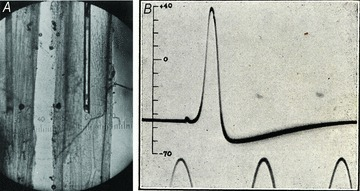
\includegraphics[width=0.5\textwidth]{ActionPotential.jpg}
\caption[Esperimento di \cite{Hodgkin1952}]
{ Sonda e misurazione del potenziale d'azione nell'assone del calamaro gigante {\it Loligo forbesi} nell'esperimento di \cite{Hodgkin1952}. In \cite{Schwiening2012}. }
\label{fig:ActionPotential}
\end{figure}


\begin{equation}
 I = C\frac{dV}{dt} + a_{K}(V-V_{K}) + a_{Na}(V-V_{Na}) + a_{l}(V-V_{l})
\end{equation}




%-----------------------------------------------------------------------
\section{La tecnologia di rilevazione CMOS-MEA}
\label{sez:Mea}\label{sez:Rilevazione}

{\it Micro Array Technology}. Si tratta di una tecnica di rilevazione e di stimolazione basata su un rivelatore piano composto di micro elettrodi utilizzata per la prima volta nel 1972 in ambito medico. Le cellule neuronali coltivate in vitro aderiscono alla superficie del rilevatore dove in prossimità degli elettrodi è sensibile al potenziale d'azione (scariche ioniche extracellulari, cfr. \ref{sez:Potenziale} ) ed è capace anche di fornire un segnale elettrico di stimolazione.

\begin{figure}%[tbp] 
\centering    
\includegraphics[width=0.5\textwidth]{Mea.png}
\caption[Rivelatore MEA]
{ (a) Layout MEA. (b) Schema microelettrodi e aperture. (c,d) MEA con coltura di cellule in una cilindro di vetro aperto sul fondo.  \cite{Kim2014}. }
\label{fig:MEA}
\end{figure}

Parametri critici dei rivelatori MEA sono la densità e l'impedenza dei micro elettrodi. I valori tipici per questi due parametri sono riportati nella tabella \ref{tab:DimensionamentoMea}.

\paragraph{Impedenza} L'impedenza dei microelettrodi dipende dalla loro area che può essere aumentata con la formazione di nanostrutture metalliche come nanotubi o nanopori che aumentano le capacità di rivelazione dei sensori \cite{Kim2014}.

\paragraph{Densità} La densità spaziale deli elettrodi nel sensore MEA può essere drasticamente aumentata con transistor CMOS integrati in un chip\footnote{Il cui disegno è effettuato con tecniche
VLSI {Very Large Scale Integration}, atte a implementare nello stesso chip di rivelazione anche i circuiti di amplificazione, multiplexing, conversione analogico-digitale e filtro}.

\begin{table}%[c]
\begin{tabular}{l|c|c|c}
{\bf Elettrodi}             & MEA                & CMOS-MEA   & NeuroChip \\ \hline

Numero                   & 512 & 16.384 & 98.304    \\
Diametro ($\mu m$)       & 20  & 20     & 5         \\
Spaziatura ($\mu m$)     & nr  & 20     & 5         \\
Rumore ($\mu V_{rms}$)   & 50  & 2.4    & 80-120    \\
Impedenza a 1$kHz$, ($k\Omega$)
                         & 30  & nr     & nr \\ 
SNR per elettrodo (dB)   & 100 & nr     & 3-7 \\
Potenza richiesta ($mW$) &  nr & 135    & nr \\
\hline
\end{tabular}
\caption[Dimensionamenti tipici MEA]
{Tecnologia MEA. Dimensionamenti tipici. Dati da \cite{Kim2014, Vallicelli2017}}
\label{tab:DimensionamentoMea}
\end{table}



%-----------------------------------------------------------------------
\section{L'algoritmo di spike sorting nell'esperimento Neuro Chip}
\label{sez:NeuroChip}

Attraverso la tecnologia presentata nelle sezioni precedenti, l'esperimento Neuro Chip riceve un segnale complesso composto da picchi di potenziale d'azione, caratterizzati approssimativamente da ampiezze di $500$ $mV$ e frequenze nell'ordine dei $kHz$, sovrapposto ad un segnale rumoroso derivante sia dalla componente tecnologica che quella biologica. L'entità del rumore varia dai $5-7dB$ $SNR$.  Fin qui l'organizzazione spaziale dei rilevatori CMOS è stata trascurata, laddove invece ognuno dei $16x192$ pixel è in grado di generare un segnale indipendente registrato ad altissima frequenza in modo da poter trattare contemporanei i segnali da pixel diversi.

L'alta risoluzione spaziale e temporale del sensore fa si che un singolo picco di potenziale sia rilevato contemporaneamente da un array di $3x3$ sensori per un intervallo temporale della durata di $3$ campioni consecutivi. Sulla base di questa sistematicità la rilevazione di un picco è basata su un test statistico del $Chi2$, in base al quale una porzione di segnale contiene un picco se la media quadratica normalizzata per la varianza del segnale è superiore ad un dato valore di soglia.

\begin{equation}
 \sum_{i,j=1,2,3} \sum_{t=0}^{2} \frac{|V_{i,j}(t)|^{2}}{\sigma_{i,j}^{2}} \geq \tau
\end{equation}

La soglia $\tau$ in un test statistico è determinata dalla dall'ampiezza desiserata del test secondo l'impostazione di Neyman e Fischer. Sulla base del contributo di \cite{Lambacher2011} nell'esperimento Neurochip, la soglia $\tau$ è determinata sperimentalmente in sede di calibrazione della strumentazione.

\begin{figure}%[tbp] 
\centering    
\includegraphics[width=0.5\textwidth]{Pixel.png}
\caption[Schema pixel esperimento Neuro chip]
{ Schema pixel esperimento Neuro chip.
Da \cite{Vallicelli2017}. }
\label{fig:Pixel}
\end{figure}
